\documentclass[11pt,a4paper]{article}
\usepackage[utf8]{inputenc}
\usepackage[T1]{fontenc}
\usepackage{amsmath,amsfonts,amssymb}
\usepackage{apacite}
\usepackage{natbib}
\usepackage{graphicx}
\usepackage{booktabs}
\usepackage{threeparttable}
\usepackage{url}
\usepackage{hyperref}
\usepackage[margin=2.5cm]{geometry}
\usepackage{setspace}
\usepackage{comment}
\onehalfspacing

\newcommand{\Var}{\text{Var}}
\newcommand{\Cov}{\text{Cov}}

% Define \sym command for significance stars from esttab
\newcommand{\sym}[1]{{#1}}

\title{Estimating the Value of CEOs in Privately Held Businesses\thanks{Project no. 144193 has been implemented with the support provided by the Ministry of Culture and Innovation of Hungary from the National Research, Development and Innovation Fund, financed under the KKP\_22 funding scheme. This project was funded by the European Research Council (ERC Advanced Grant agreement number 101097789). The views expressed in this research are those of the authors and do not necessarily reflect the official view of the European Union or the European Research Council. \emph{Author contributions:} Conceptualization and study design: Koren, Orbán and Telegdy. Data curation, integration and quality assurance: Szilágyi and Vereckei. Statistical analysis: Koren and Telegdy. Writing the original draft: Koren. Review and editing: Koren, Orbán and Telegdy.}}

\author{Miklós Koren\thanks{Central European University, HUN-REN Centre for Economic and Regional Studies, CEPR and CESifo. E-mail: korenm@ceu.edu} \\
        Krisztina Orbán\thanks{Monash University.} \\
        Bálint Szilágyi\thanks{HUN-REN Centre for Economic and Regional Studies.} \\
        Álmos Telegdy\thanks{Corvinus University of Budapest.} \\
        András Vereckei\thanks{HUN-REN Centre for Economic and Regional Studies, Institute of Economics.}}

\date{\today}

\begin{document}

\maketitle

\begin{abstract}
We estimate CEO value in private firms using Hungarian administrative data covering over one million firms and CEOs from 1992-2022. Our model separates owner-controlled inputs (capital, location) from CEO-controlled inputs (labor, materials). We introduce a placebo-controlled event study comparing actual CEO transitions to randomly assigned fake transitions in stable firms. Raw estimates suggest [[raw CEO effect]] percent performance differences between good and bad CEOs, but [[placebo effect]] percent is mechanical noise. The true causal effect is [[true CEO effect]] percent—only [[true effect as percent of raw]] percent of the raw correlation. Three-quarters of apparent CEO variation is spurious, explaining weak results in studies using manager fixed effects as explanatory variables.
\end{abstract}

\textbf{Keywords:} CEO value, private firms, productivity

\textbf{JEL Classification:} [To be added]

\newpage

%%%%%%%%%%%%%%%%%%%%%%
\section{Introduction}
%%%%%%%%%%%%%%%%%%%%%%

To what extent do CEOs contribute to firm performance? Good management can improve firm productivity, as suggested by interventions that improve management practices \citep{bloom2013does}, training programs that build capabilities \citep{mckenzie2021small}, or leadership changes that reshape organizations \citep{Bertrand2003-io,bennedsen2020ceos,metcalfe2023managers}. Quantifying individual CEO contribution is complicated because modern businesses rely on a variety of inputs: tangible and intangible capital (plants, production lines, technical and organizational know-how, brand value), labor, intermediate inputs, and raw materials. Among these, only managerial capital is under CEO control, and its effects are difficult to isolate from other inputs.

Starting from \citet{Bertrand2003-io}, event studies around CEO changes attribute all changes in observable business policies to leadership changes. In public companies with dispersed ownership, CEOs and boards of directors have broad power in running the business. In private firms, ownership concentration gives owners direct control over strategic choices, creating a division of decision rights that blurs attribution of outcomes to CEOs versus owners \citep{fama1983separation, jensen1976theory, burkart2003family}. Owners may have primary decision rights on large investment projects, branding, and acquisitions. This distinction is empirically important: \citet{quigley2022ceo} find CEO effects are nearly twice as large in Swedish private firms compared to public ones, though our results suggest much of this apparent effect is noise. Accurately measuring CEO contribution in private businesses is important for studying the manager market and executive pay practices. Recent work has compared CEO pay to CEO value in public firms \citep{tervio2008difference,gabaix2008ceo}, but similar analysis for private firms remains limited.

We make three contributions. First, we develop a model that accounts for the division of control between owners who set fixed inputs (tangible and intangible capital) and CEOs who optimize variable inputs (labor, materials). This framework clarifies what CEOs can and cannot affect, enabling cleaner identification of their contribution. Second, we assemble comprehensive administrative data covering the universe of Hungarian firms and their CEO networks over three decades (1992-2022), tracking over [[total firms]] firms and [[total CEOs]] CEOs. Third, we introduce a placebo-controlled event study design that separates true CEO effects from the mechanical noise that contaminates fixed effects estimates when managers have short tenures.

Our modeling approach treats CEOs in private firms as plant managers responsible for operational decisions. This simplification underestimates their strategic importance but provides a better approximation than models of superstar CEOs in public companies. This characterization aligns with evidence from family firms where professional managers face constraints on strategic decisions while maintaining operational autonomy \citep{zellweger2012managing}, and with studies of multi-plant firms where headquarters retains capital allocation authority while delegating production decisions to plant managers \citep{bloom2012americans}.

Comprehensive administrative data from Hungary offers several advantages. Mandatory registration of all company directors, including CEOs, ensures complete coverage without selection bias. The transition economy context likely features greater variation in managerial quality than mature markets, enhancing statistical power. The large sample size and long time span enable construction of CEO mobility networks essential for identification. The institutional context matters: \citet{crossland2011differences} show that national institutions affect CEO discretion, with civil-law countries like Hungary typically granting less managerial autonomy than common-law systems, making our owner-CEO division particularly relevant.

Because CEO tenures in our data are short, estimated CEO effects contain substantial noise from averaging residual productivity shocks over few observations. This small-sample bias, known in the labor economics literature as ``limited mobility bias'' \citep{andrews2008high}, complicates interpretation of fixed effects estimates. To address this, we introduce a placebo-controlled event study design.

To illustrate our approach, consider a firm with the same CEO from 2000-2010. We randomly assign a fake transition in 2005, creating two pseudo-CEOs. If estimated `effects' for these pseudo-CEOs diverge substantially, this reveals the noise problem in fixed effects estimation. By comparing actual CEO transitions to these placebo transitions, we can correct the fixed effects estimates for noise, isolating the true CEO contribution.

Our headline result challenges conventional wisdom about CEO importance. The naive comparison suggests firms hiring good CEOs outperform those hiring bad CEOs by [[raw CEO gap]] percent—a large effect consistent with the view that leadership quality is paramount. However, our placebo control reveals [[placebo gap]] percent of this difference arises from noise in the estimation process, not skill differences. The true causal effect of CEO quality is [[true CEO effect]] percent: economically meaningful but only [[true as percent of raw]] percent of what raw correlations suggest. Three-quarters of apparent variation in CEO quality is spurious.

Our work connects to the broader literature on management practices and firm productivity. Randomized controlled trials demonstrate that management training and consulting improve firm performance \citep{bloom2013does}, but these interventions change practices rather than people. Whether replacing managers generates similar gains remains contentious. Evidence from public sector organizations suggests modest manager effects \citep{fenizia2022managers, janke2024role}, while studies of family firms find larger impacts when professional managers replace family members \citep{bennedsen2007inside}. Our results for private firms fall between these extremes: CEOs matter, but less than raw correlations suggest.

Methodologically, our paper builds on the two-way fixed effects literature in labor economics that decomposes wages into worker and firm components \citep{Abowd1999Econometrica, Card2018JoLE}. These studies face similar challenges from limited mobility creating small-sample bias \citep{andrews2008high} and have developed bias-correction methods \citep{Bonhomme2023-dx, gaure2014correlation}. We adapt this framework to the CEO-firm setting but add placebo controls to separate signal from noise. This approach is valuable when studying managers who, unlike workers, have few observations per individual, making traditional bias-correction methods less effective. Recent work has documented apparently increasing CEO effects over time \citep{quigley2015has}, but these studies do not account for the mechanical noise we identify. \citet{lippi2014corporate} find that concentrated ownership in Italian firms distorts executive selection and reduces productivity by 10\%, providing motivation for our framework separating owner and CEO decisions.

%%%%%%%%%%%%%%%%%%%%%%%%%%%%%%%%%%
\section{A Model of Production with Owner- and Manager-Controlled Inputs}
%%%%%%%%%%%%%%%%%%%%%%%%%%%%%%%%%%%

Our model highlights a key institutional feature of private firms: the separation of strategic decisions (owner-controlled) from operational decisions (manager-controlled).\footnote{Both theoretical results \citep{fama1983separation, jensen1976theory, burkart2003family, schulze2021property} and empirical evidence \citep{durand2003ownership, gao2015comparison, quigley2022does, cole2008privately, nakazato2011executive, gompers2023market, bloom2012organization, wang2019decentralization, buffington2017mops} confirm that in privately held firms and firms with concentrated ownership, managerial discretion on strategic decisions is limited and owner control dominates.} This division of decision rights, common in private businesses, affects how we identify manager effects: we cannot control for variable inputs when estimating manager productivity because variable input levels are an outcome of manager decisions and are correlated with productivity.\footnote{A similar point was made by \citet{Gandhi2020-nu}, who emphasize that freely adjustable inputs are ``bad controls'' because they are determined by productivity.} 

Firms produce output using a Cobb-Douglas production function with both fixed and variable inputs. The production function for firm $i$ with manager $m$ at time $t$ is:
\begin{equation}\label{eq:production}
Q_{imt} = A_i Z_{m} \varepsilon_{it} K_{it}^\alpha L_{imt}^{\beta} M_{imt}^{\gamma}
\end{equation}
where $A_i$ represents time-invariant organizational capital (location, brand value, customer relationships), $Z_m$ captures manager skill, $\varepsilon_{it}$ is residual productivity, $K_{it}$ is physical capital, $L_{imt}$ is labor input, and $M_{imt}$ is intermediate input usage. 

Standard production function estimation combines the first three components into a single measure: $\Omega_{it} = A_i Z_m \varepsilon_{it}$, called total factor productivity (TFP). Our framework decomposes TFP into firm-specific advantages ($A_i$), manager-specific skill ($Z_m$), and residual productivity shocks ($\varepsilon_{it}$) to identify the manager contribution.

We assume physical capital investment ($K_{it}$) and organizational assets ($A_i$), including location choices, brand development, and CEO hiring decisions are predetermined. Managers control labor hiring ($L_{imt}$) and input purchases ($M_{imt}$). 

The production function exhibits decreasing returns to scale in variable inputs ($\beta + \gamma < 1$), which pins down optimal firm size even under perfect competition. Fixed inputs $A_i$ and $Z_m$ create firm-specific and manager-specific advantages that generate economic rents.

Managers maximize profit by choosing variable inputs optimally given the predetermined choices. Under sector-specific output price $P_{st}$, wage rate $W_{st}$, and material price $\varrho_{st}$, the first-order conditions yield closed-form solutions for optimal input demands. Substituting these back into the revenue function gives:
\begin{equation}\label{eq:revenue}
R_{imst} = (P_{st}A_i Z_m \varepsilon_{it})^{1/\chi}
K_{it}^{\alpha/\chi}
W_{st}^{-\beta/\chi}
\varrho_{st}^{-\gamma/\chi}
(1-\chi)^{(1-\chi)/\chi}
\end{equation}
Revenue increases in manager skill $Z_m$, organizational capital $A_i$, and physical capital $K_{it}$, while decreasing in input prices. The elasticity of revenue with respect to manager skill is $1/\chi > 1$, with $\chi := 1 - \beta - \gamma$, the share of surplus in revenue. 

The surplus accruing to fixed factors (factors other than labor and materials), which owners and managers jointly maximize, equals revenue minus payments to variable inputs:
\begin{equation}\label{eq:surplus}
S_{imst} = R_{imst} - W_{st}L_{imt} - \varrho_{st}M_{imt} = \chi R_{imst}
\end{equation}
Under Cobb-Douglas technology, surplus is a constant fraction $\chi$ of revenue. This proportionality allows us to work directly with revenue, simplifying estimation while preserving economic insights. Taking logarithms of the revenue equation:
\begin{equation}\label{eq:log_revenue}
r_{imst} = C+\frac{\alpha}{\chi} k_{it} + \frac{1}{\chi} z_{m} + \frac{1}{\chi} a_i + \frac{1}{\chi} p_{st} + \frac{1}{\chi}\epsilon_{it} 
- \frac{\beta}{\chi} w_{st} - \frac{\gamma}{\chi} \rho_{st}
\end{equation}
where lowercase letters denote logarithms (e.g., $\epsilon_{it} = \log \varepsilon_{it}$) and $C$ is a constant.

The value of replacing manager $m$ with manager $m'$ at the same firm is the extent to which surplus changes as the manager changes:
\begin{equation}\label{eq:manager_value}
r_{im'st} - r_{imst} = \frac{1}{\chi}(z_{m'} - z_{m})
\end{equation}
Manager value equals the skill difference scaled by $1/\chi$. This scaling reflects a leverage effect: a 1\% better manager hires more variable inputs, thereby increasing revenue and surplus by more than 1\%.

Our model abstracts from corporate governance frictions that could lead managers to make suboptimal decisions. These frictions are less problematic in concentrated ownership settings where owners retain control over strategic choices. While agency problems may affect long-term vision, risk-taking, and entrepreneurship, the incentive to increase revenue and reduce operating costs remains aligned between owners and managers in most private firms.

The model excludes dynamic considerations such as adjustment costs or forward-looking behavior. Strategic decisions are forward-looking due to their persistence, but we treat them as predetermined from the manager's perspective. Even though the optimization framework is static, our empirical application allows for arbitrary time-series correlation within and across variables. The data validate this choice: strategic variables like capital evolve slowly with little correlation to manager changes, while operational variables adjust immediately following CEO transitions.

\section{Corporate Data from Hungary}

Hungary provides an ideal setting for studying CEO effects in private firms. The country offers complete administrative data coverage for all incorporated businesses with mandatory CEO registration, spanning 30 years from the transition economy of the 1990s through EU accession in 2004 to the present. This coverage enables us to track CEO careers across firms and construct mobility networks necessary for identification.

Hungary provides three advantages: (1) mandatory registration of all directors, including CEOs, (2) no selection into coverage as all incorporated firms must report, and (3) a transition economy where CEO quality variation is likely larger than in mature markets, providing greater statistical power. The large-scale economic transformation following 1990 created substantial heterogeneity in managerial practices and quality, ideal for identifying CEO effects. 

Our analysis combines two administrative datasets. The firm registry, maintained by Hungarian corporate courts, contains records on all company representatives—individuals authorized to act on behalf of firms. These records include CEOs and other executives with signatory rights, tracked through a temporal database where each entry reflects representation status over specific time intervals. Updates occur when positions change, personal identifiers are modified, or reporting standards evolve. The registry provides names, addresses, dates of birth (from 2010), and mother's names (from 1999), though numerical identifiers exist only from 2013 onward.

The balance sheet dataset contains annual financial reports for all Hungarian firms required to file statements. This includes sales revenue, export revenue, employment counts, tangible and intangible assets, raw material and intermediate input costs, personnel expenses, and indicators for state and foreign ownership. The two datasets cover [[total firms]] firms over [[total years]] years, yielding [[total firm-years]] firm-year observations before sample restrictions.

Constructing a panel of CEOs requires resolving two questions: what constitutes a firm and who qualifies as a CEO. For firms, we track legal entities through time using tax identifiers, which remain stable despite occasional reuse ([[tax ID reuse percent]]\% of cases). Mergers and acquisitions create new entities in our framework—we follow legal entities rather than economic conglomerates.

Identifying individual CEOs poses greater challenges. Before 2013, no numerical identifiers existed, requiring entity resolution based on names, addresses, mother's names, and birthdates. We link records across these dimensions to create unique person identifiers, enabling tracking across firms and over time. Matching quality improves after 1999 (when mother's names reporting commences) and 2010 (when birthdates reporting starts), though the 1990s data achieves reasonable coverage through name and address matching. 

CEO identification within firms requires heuristics since job titles are inconsistently recorded. When explicit ``managing director'' titles exist ([[managing director percent]]\% of cases), we use them directly. For remaining cases, we assume all representatives are CEOs if three or fewer exist at the firm. When more than three representatives are present, we assign CEO status based on continuity with previously identified CEOs. Time spans between appointments are often unclosed or non-contiguous, requiring imputation based on sequential information, assuming representatives remain active if their tenure includes June 21 of each year.

We apply several restrictions to create a sample suitable for productivity analysis. First, we exclude mining and finance sectors due to specialized accounting frameworks and regulatory environments. Second, we drop firms ever having more than [[max simultaneous CEOs]] simultaneous CEOs (removing [[dropped for multiple CEOs]] observations) to avoid complex governance structures that complicate identification. Third, we exclude firms with more than [[max CEO changes]] CEO changes over the sample period ([[dropped for excess changes]] observations) to reduce noise from misclassified transitions. Fourth, we remove all state-owned enterprises, as their objectives and constraints differ from private businesses \citep{orban2019inception}.

Most importantly, we restrict attention to firms that employ at least [[min employees]] workers at some point in the firm lifecycle. This filter removes [[percent dropped for size]] of observations but eliminates shell companies, tax optimization vehicles, and self-employment arrangements masquerading as corporations. The remaining firms represent genuine businesses with meaningful economic activity where management quality affects performance.

We exclude public firms and joint-stock companies from our analysis. The few companies traded on the Budapest Stock Exchange operate under different governance structures, compensation schemes, and disclosure requirements than private businesses. We also exclude cooperatives and other non-standard corporate forms where multiple managing directors share executive authority, as these organizational structures complicate identification of individual CEO effects.

\begin{table}[htbp]
\centering
\caption{Sample Over Time}
\label{tab:sample}
\begin{tabular}{*{6}{c}}
\toprule
Year & \shortstack{Total\\firms} & \shortstack{Sample\\firms} & CEOs & \multicolumn{2}{c}{Connected component} \\
\cmidrule(lr){5-6}
 & & & & Firms & CEOs \\
\midrule
1992 &       98,780 &       25,833 &       31,746 &        1,423 &        1,713 \\
1995 &      171,759 &       45,828 &       53,704 &        2,659 &        3,028 \\
2000 &      280,386 &       73,837 &       83,862 &        4,783 &        5,100 \\
2005 &      326,905 &       92,242 &      104,380 &        6,283 &        6,474 \\
2010 &      384,570 &      103,892 &      116,680 &        7,405 &        7,084 \\
2015 &      433,371 &      116,543 &      124,960 &        8,332 &        7,488 \\
2020 &      424,501 &      115,755 &      123,504 &        7,789 &        6,841 \\
2022 &      454,106 &      113,387 &      121,730 &        7,419 &        6,509 \\
\midrule
Total &    1,063,172 &      217,737 &      339,993 &       14,416 &       22,001 \\
\bottomrule
\end{tabular}
\begin{minipage}{12cm}
\footnotesize
\textit{Notes:} This table presents the evolution of the sample from 1992 to 2022. Column (1) shows the total number of distinct firms with balance sheet data. Column (2) shows the number of distinct firms after applying data quality filters. Column (3) shows the number of distinct CEOs. Columns (4) and (5) show the subset of distinct firms and CEOs that belong to the largest connected component of the manager network, where managers are connected if they have worked at the same firm. The table shows every fifth year plus the first year (1992), last year (2022), and totals of distinct counts. \end{minipage}
\end{table}


[[QUESTION: Are we reporting largest component or all components above size N?]]

[[TODO: Explain size of connected components]

Given the 1990s' rapid economic liberalization, transition to market economy, and foreign direct investment inflows, we conducted robustness checks restricting the sample to post-2004 data following Hungary's EU accession. The results remain unchanged, confirming our findings are not driven by the transition period's institutional environment.

The resulting sample contains distinctive patterns of CEO demographics and tenure. Among CEOs in our analysis sample, [[percent Hungarian names]]\% have Hungarian names (verified algorithmically), with only [[percent foreign names]]\% foreign. Gender identification among Hungarian-named CEOs reveals [[percent male]]\% male representation. Remarkably, [[percent founders]]\% of CEOs were present at their firm's founding, highlighting the prevalence of founder-managers in private businesses.

CEO mobility creates networks essential for fixed effects identification. [[percent multiple firms]]\% of CEOs manage multiple firms during the sample period, generating connections between firms. The largest connected component of the bipartite firm-CEO network contains [[connected component size]] managers and a comparable number of firms—[[percent in component]]\% of all managers but representing a substantial share of economic activity. This connected component enables comparison of CEO effects within a common reference frame, though it raises questions about representativeness we address in robustness checks.

[[Note: Connected component firms are significantly larger than the full sample, with [[connected revenue premium]] higher log revenue on average. as we argue below, this does not affect our results. ]]

CEO tenure varies across firms. While [[percent single CEO firms]]\% of firms retain the same CEO throughout their observed lifetime, the remaining firms experience leadership transitions that enable identification. Among firm-years with CEO information, [[percent single CEO firm-years]]\% have single CEOs, [[percent two CEO firm-years]]\% have two, and [[percent multiple CEO firm-years]]\% have more (before our sample restrictions). CEO spell lengths follow an exponential distribution with a [[annual hazard rate]]\% annual hazard rate, implying typical tenures of [[typical tenure range]] years.


\begin{table}[htbp]
\centering
\caption{CEO Patterns and Spell Length Analysis}
\label{tab:ceo_patterns}

\centering
\begin{tabular}{cc}
    \begin{minipage}{0.45\textwidth}
        \textbf{Panel A: Number of CEOs per Firm}
        \begin{tabular}{lcc}
\toprule
CEOs & Firm-Year & Firm \\
\midrule
1 & 79\% & 79\% \\
2 & 18\% & 17\% \\
3 & 3\% & 3\% \\
4+ & 1\% & 1\% \\
Total &    1,884,566 &      402,875 \\
\bottomrule
\end{tabular}

    \end{minipage} &
    \begin{minipage}{0.45\textwidth}
        \textbf{Panel B: Spell Length Distribution}
        \begin{tabular}{lcc}
\toprule
Length & Actual & Placebo \\
(Years) & Spells & Spells \\
\midrule
1 & 22\% & 27\% \\
2 & 15\% & 19\% \\
3 & 11\% & 14\% \\
4+ & 51\% & 40\% \\
Total &      107,957 &       14,978 \\
\bottomrule
\end{tabular}

    \end{minipage}
\end{tabular}

\begin{minipage}{12cm}
\footnotesize
\textit{Notes:} Panel A shows the distribution of CEO counts per firm across firm-years and firms. Panel B compares the spell length distribution between actual CEO transitions and synthetically generated placebo transitions. The similar distributions validate our placebo methodology.
\end{minipage}
\end{table}

[[Krisztina: In \ref{tab:industry_stats} did we want to remove the reference to EBITDA? Also, should mining and finance be in table as they are excluded form the analysis?]]

\section{Estimation}

Our estimation proceeds in four steps: measuring the surplus share (the share of revenue accruing to fixed factors), estimating the revenue function, recovering manager fixed effects, and validating causality through event studies. Each step builds toward separating true CEO effects from the noise that contaminates raw estimates.

\paragraph{Step 1: Measuring the Surplus Share.} The parameter $\chi$---the share of surplus in revenue---determines how manager skill translates into firm performance. Under Cobb-Douglas technology, this share equals one minus the combined revenue shares of labor and materials. Following \citet{Gandhi2020-nu}, we measure $\chi$ from the data as:
\begin{equation}
\hat{\chi}_s = 1 - \frac{\sum_{i \in s}(W_{st}L_{it} + \varrho_{st}M_{it})}{\sum_{i \in s} R_{it}}
\end{equation}
where the summation runs over firms in sector $s$. This approach yields sector-specific estimates of $\chi$. The $1/\chi$ scaling in our framework creates a leverage effect where manager skill is amplified in its impact on firm performance.

\paragraph{Step 2: Estimating the Revenue Function.} With $\hat{\chi}$ measured, we estimate the revenue function to recover the capital elasticity and control for observable factors. Using lowercase letters for logarithms, the estimating equation is the empirical counterpart of (\ref{eq:log_revenue}):
\begin{equation}
r_{imst} = \frac{\alpha}{\chi} k_{it} + \frac{1}{\chi}z_m + \lambda_i + \mu_{st} + \tilde{\epsilon}_{it}
\end{equation}
where $r_{imst} = \log R_{imst}$ is log revenue, $k_{it} = \log K_{it}$ is log capital, $\lambda_i$ captures firm fixed effects, $\mu_{st}$ are sector-year fixed effects, and $\tilde{\epsilon}_{it} = \epsilon_{it}/\chi$ is rescaled residual productivity. We include controls for firm age, intangible asset presence, and foreign ownership, though these minimally affect the capital coefficient.

The key assumptions are: (1) all firms within a sector face the same prices, and (2) for each manager, residual productivity $\tilde{\epsilon}_{it}$ has zero mean when averaged across all their firms and time periods: $E[\bar{\epsilon}_m] = 0$ where $\bar{\epsilon}_m = \frac{1}{N_m}\sum_{i,t \in m} \tilde{\epsilon}_{it}$ and the sum runs over all firm-year observations under manager $m$.

We do not require random manager mobility or that residual productivity has zero mean at the point of CEO transition. Manager assignment can be endogenous: good managers may systematically move to firms experiencing positive shocks or be hired when firms anticipate improvements. We only require that these shocks average to zero over a manager's entire career. This is a weaker assumption than random assignment but still substantive: it rules out managers who systematically arrive at permanently improving (or declining) firms.

We estimate using OLS with high-dimensional fixed effects via \texttt{reghdfe} \citep{reghdfe}. The coefficient on log capital is $\hat{\alpha}/\hat{\chi}$, which we multiply by $\hat{\chi}$ to recover $\hat{\alpha}$.

\paragraph{Step 3: Recovering Manager Fixed Effects.} After estimating the revenue function, we compute log total factor productivity by removing the contribution of capital and sectoral prices from revenue:
\begin{equation}
\omega_{imst} = \hat{\chi} r_{imst} - \hat{\alpha} k_{it} - \hat{\mu}_{st} = z_m + \lambda_i + \epsilon_{it}
\end{equation}
This measure of log TFP contains manager skill, firm effects, and residual productivity. In standard production function estimation, this entire term would be treated as a single TFP measure. Our decomposition separates the manager contribution from other sources of productivity.

We estimate a two-way fixed effects model with firm and manager fixed effects. Our identification relies on the zero-mean condition described above: residual productivity must average to zero for each manager across their career. This allows for various forms of endogenous mobility but rules out systematic patterns where managers consistently join permanently improving or declining firms. 

The event study provides a diagnostic test for this identification assumption. Pre-trends in productivity before CEO transitions would suggest (though not prove) that the zero-mean assumption is violated. If productivity systematically rises before good CEOs arrive, we worry that the positive trend continues post-transition, violating $E[\bar{\epsilon}_m] = 0$. Conversely, the absence of pre-trends makes it harder to construct plausible endogeneity stories. While we cannot rule out contemporaneous shocks that coincide exactly with CEO changes (e.g., owners simultaneously firing the CEO and adopting new technology), such precise timing is less plausible than gradual changes that would manifest as pre-trends. Our event studies show no significant pre-trends, supporting but not proving our identification assumption. The absence of strong pre-trends in our data contrasts with evidence from \citet{cornelli2013monitoring} showing boards actively monitor and replace CEOs when performance deteriorates in public firms, suggesting our private firm transitions may be less performance-driven. While \citet{jenter2021performance} find 38-55\% of turnovers are performance-induced in U.S. public firms, our private firm setting likely features more random CEO transitions given the absence of market pressures and board oversight.

The system of fixed effects is identified only within connected components: groups of firms and managers linked through mobility. Two managers can be compared if they worked at the same firm or connect through a chain of shared employment relationships. We can estimate $\hat z_m$ for every manager, but only up to a constant term that may vary across connected components. 


Our largest connected component contains [[connected component size]] managers, enabling comparisons within this network. We normalize the manager effect to be mean zero in the largest connected component.

The connected component represents a non-random subset of the economy, with member firms larger than average. This selection is not problematic for our identification strategy since we allow manager effects to correlate arbitrarily with observable characteristics. We cannot extend the analysis to singleton firms or disconnected components where manager fixed effects lack a common reference point for interpretation.

\paragraph{Step 4: Placebo-Controlled Event Studies.} Even when $\epsilon$ is orthogonal to $z$, estimated fixed effects contain substantial small-sample noise when manager transitions are infrequent and manager tenures are short.\footnote{Worker-firm fixed effect studies face similar challenges called ``limited mobility bias'' \citep{andrews2008high} and have developed bias-correction methods \citep{Bonhomme2023-dx, gaure2014correlation}.}

To understand the sources of small-sample bias and how we address it, we remove the firm fixed effect from TFP by subtracting the firm average:
\begin{equation}
\Delta\omega_{imt} = \Delta z_{m_{it}} + \Delta\epsilon_{it},
\end{equation}
where $\Delta x_{it} := x_{it} - \frac{1}{N_i}\sum_{\tau} x_{i\tau}$ denotes the deviation of a variable from its within-firm mean. When a firm changes CEOs, the change in log TFP captures both the true skill difference and accumulated noise. The noise component---the average of residual productivity shocks during each manager's tenure---dominates the signal when tenures are short. 

Our solution leverages a simple insight: when CEOs do not change, we still observe variation in log TFP driven purely by noise:
\begin{equation}
\Delta\omega_{imt} = \Delta\epsilon_{it}.
\end{equation}
By applying the same estimation procedure to ``non-changes,'' we can measure and filter out the noise component.

We construct placebo CEO transitions in three steps. First, we estimate the time-varying hazard of actual CEO changes. Second, we identify firms with long CEO tenures (7+ years) where no actual change occurs. Third, we randomly assign placebo transitions to these stable firms using the estimated hazard function.

For instance, a firm with the same CEO from 1992-2000 might receive a placebo transition in 1996, artificially splitting the tenure into two pseudo-CEOs. The timing follows the empirical hazard, ensuring the mechanical noise properties—averaging residual productivity over varying tenure lengths—match between actual and placebo groups.

To validate our placebo methodology, we verify that synthetically generated CEO transitions match actual patterns. Taking firms with stable leadership (same CEO for [[min stable tenure]]+ years), we randomly assign placebo transitions using the empirical hazard function. The resulting spell length distribution mirrors actual CEO changes: [[percent one year spells]]\% last one year, [[percent two year spells]]\% two years, declining thereafter. This similarity confirms our placebo transitions capture realistic turnover dynamics while maintaining the property that no skill change occurs.

We implement the event study around CEO transitions at time $g$, comparing actual changes (treatment) to placebo changes (control):
\begin{equation}
\omega_{imt} = a_i + \gamma_{t-g} + \epsilon_{it}
\end{equation}
The coefficients $\gamma_{t-g}$ capture the evolution of log TFP in event time, where $t-g \in [-4, 3]$ and we normalize $\gamma_{-1} = 0$.

Because both groups receive a ``treatment'' (actual or placebo), standard difference-in-differences cannot be used. We adapt the \citet{Callaway2021JoLE} estimator for two treatment types using the \texttt{xt2treatments} package \citep{Koren2024xt2treatments}. The key innovation is precisely aligning transitions in event time—both actual and placebo changes occur at $t=0$, enabling a clean comparison of dynamics between treated and control firms.


%%%%%%%%%%%%%%%%%
\section{Results}
%%%%%%%%%%%%%%%%%

\subsection{Production Function Estimates}

Table \ref{tab:surplus_share} in the Appendix reports our estimates of the surplus share $\chi$ by industry. The estimates range from [[chi min]] to [[chi max]] across sectors, with wholesale, retail, and transport showing the lowest values and professional services the highest. These estimates imply that a 1\% increase in TFP increases revenue by [[revenue amplification range]] percent through the leverage effect of scaling variable inputs.

Table \ref{tab:revenue_function} presents the revenue function estimates. We include controls for log capital, firm age, presence of intangible assets, and foreign ownership, along with firm-CEO and sector-year fixed effects. The capital coefficient is precisely estimated at [[capital coefficient]] (standard error [[capital SE]]), consistent with capital's limited but significant role in private businesses. The intangible asset dummy shows a positive coefficient of [[intangible coefficient]], while foreign ownership contributes [[foreign coefficient]] to log revenue. Firm age exhibits diminishing returns with a coefficient of [[age coefficient]] on log age. These controls explain [[R-squared]] of the variation in log revenue. Robustness checks varying the control set and sample restrictions, reported in the Appendix, yield similar estimates.

Founder-managed firms exhibit lower revenue conditional on owner inputs, implying lower total factor productivity—consistent with evidence that family firms sacrifice growth for control \citep{bennedsen2007inside}. The performance penalty from family succession is well-documented, with heir CEOs reducing ROA by 6 percentage points in Danish firms \citep{bennedsen2007family}. Our preferred specifications focus on founder-to-outsider transitions where the separation of ownership and management is clearest. Excluding owner-managed firms yields stronger results, with one-third of the raw correlation representing true effects rather than one-quarter in the full sample. When we restrict the analysis to never-founder-managed firms, point estimates remain similar though confidence intervals widen due to the reduced sample of 834 firms, confirming our main finding of substantial noise contamination is not an artifact of founder-specific dynamics.


\begin{table}[htbp]\centering
\def\sym#1{\ifmmode^{#1}\else\(^{#1}\)\fi}
\caption{Surplus Function Estimation Results}
\begin{tabular}{l*{6}{c}}
\toprule
                    &\multicolumn{1}{c}{(1)}&\multicolumn{1}{c}{(2)}&\multicolumn{1}{c}{(3)}&\multicolumn{1}{c}{(4)}&\multicolumn{1}{c}{(5)}&\multicolumn{1}{c}{(6)}\\
                    &\multicolumn{1}{c}{Revenue}&\multicolumn{1}{c}{EBITDA}&\multicolumn{1}{c}{Wagebill}&\multicolumn{1}{c}{Materials}&\multicolumn{1}{c}{Revenue}&\multicolumn{1}{c}{Revenue}\\
\midrule
Fixed assets (log)  &       0.272\sym{***}&       0.263\sym{***}&       0.251\sym{***}&       0.323\sym{***}&       0.260\sym{***}&       0.271\sym{***}\\
                    &     (0.002)         &     (0.002)         &     (0.002)         &     (0.002)         &     (0.002)         &     (0.034)         \\
\addlinespace
Has intangible assets&       0.140\sym{***}&       0.085\sym{***}&       0.155\sym{***}&       0.165\sym{***}&       0.135\sym{***}&       0.212\sym{**} \\
                    &     (0.004)         &     (0.005)         &     (0.004)         &     (0.005)         &     (0.004)         &     (0.089)         \\
\addlinespace
Foreign owned       &       0.051\sym{***}&       0.017         &       0.086\sym{***}&       0.044\sym{**} &       0.059\sym{***}&       0.167         \\
                    &     (0.015)         &     (0.017)         &     (0.015)         &     (0.019)         &     (0.015)         &     (0.238)         \\
\midrule
Observations        &     1169474         &      927037         &     1157713         &     1184973         &     1169474         &        4122         \\
\bottomrule
\multicolumn{7}{l}{\footnotesize Standard errors in parentheses}\\
\multicolumn{7}{l}{\footnotesize All models include firm-CEO-spell fixed effects and industry-year fixed effects. Outcome variables are}\\
\multicolumn{7}{l}{\footnotesize log-transformed. Models (5) and (6) include quadratic controls for firm age and CEO tenure.}\\
\multicolumn{7}{l}{\footnotesize Model (6) restricts to largest connected component.}\\
\multicolumn{7}{l}{\footnotesize \sym{*} \(p<0.10\), \sym{**} \(p<0.05\), \sym{***} \(p<0.01\)}\\
\end{tabular}
\end{table}


The stability of our estimates across samples validates the connected component analysis. Revenue function coefficients are nearly identical when estimated on the connected component versus the full sample (Table 3, Model 6), suggesting production technology and manager effects operate similarly across both groups. While selection into the connected component is non-random—these firms are larger and hire external managers more often—the economic relationships appear invariant to this selection, supporting our use of the connected component to identify manager fixed effects.

\subsection{Raw Manager Effects and Their Distribution}

After removing the contribution of capital and other controls from revenue, we estimate manager fixed effects within the largest connected component. Figure \ref{fig:manager_distribution} shows the distribution of these estimated effects. The raw dispersion is substantial: the interquartile range spans [[IQR]] log points, suggesting that moving from a 25th percentile to a 75th percentile CEO would increase firm productivity by [[raw IQR productivity difference]] percent. Most of this variation reflects noise rather than true skill differences.

\begin{figure}[htbp]
\centering
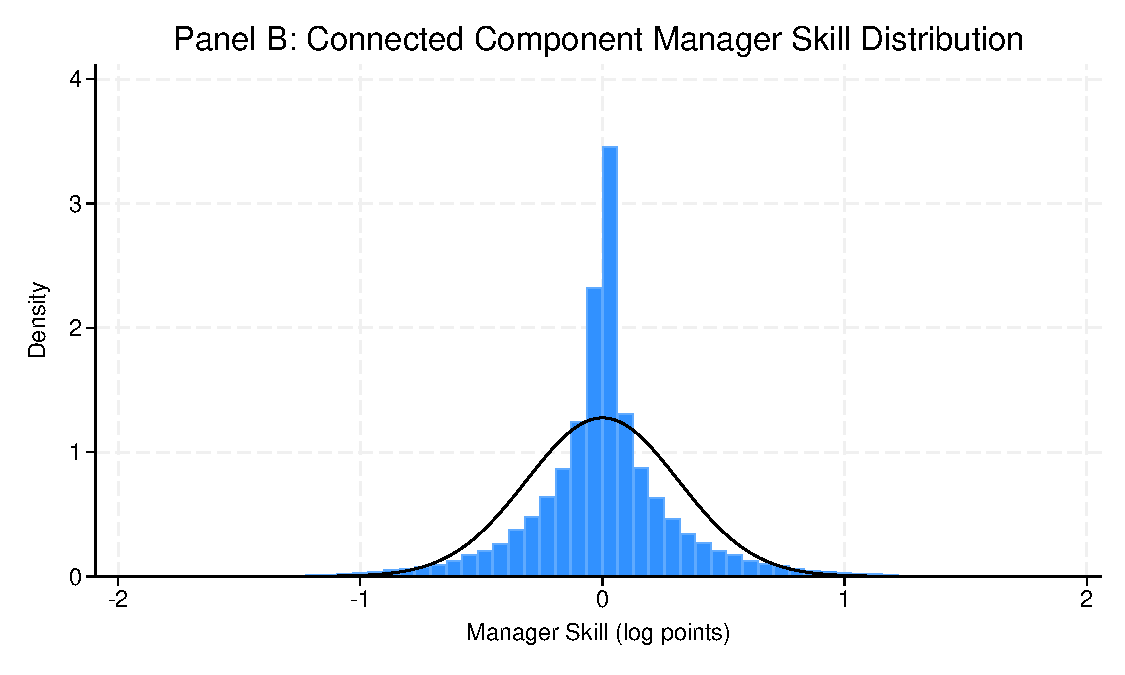
\includegraphics[width=0.8\textwidth]{figure/manager_skill_connected.pdf}
\caption{Distribution of Manager Fixed Effects in the Connected Component}
\label{fig:manager_distribution}
\end{figure}

\subsection{The Placebo Test}

To examine the dynamics of firm performance around CEO transitions, we implement an event study analysis. Figure \ref{fig:event_study_main} presents our placebo-controlled approach across different samples, where year 0 marks the first year of the new CEO.

[[Note: Replace Figure 1 with four-panel structure:
Panel (a): Raw vs Placebo for all transitions - shows how placebo captures pre-trends and mechanical jumps
Panel (b): True effect of good vs bad CEOs after placebo correction - main result
Panel (c): Post-2004 robustness - excludes transition economy period
Panel (d): Outsider-to-outsider transitions - cleanest identification without ownership changes]]

\begin{figure}[htbp]
\centering
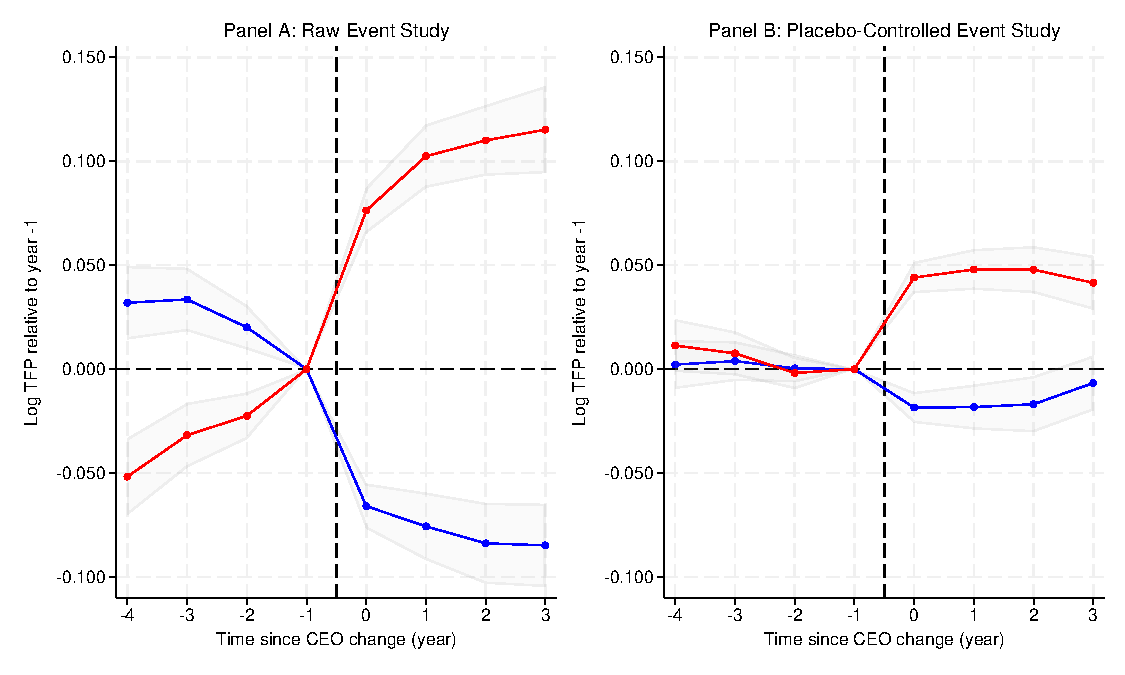
\includegraphics[width=\textwidth]{figure/event_study.pdf}
\caption{Placebo-Controlled Event Studies of CEO Transitions}
\label{fig:event_study_main}
\end{figure}

[[Note: Describe Panel (a) showing raw actual transitions exhibit large apparent effects that are largely matched by placebo transitions with no real CEO change, demonstrating the mechanical noise problem. Pre-trends visible in both actual and placebo transitions show these are not causal but arise from selection on averaged residual productivity.]]

[[Note: Describe Panel (b) showing the true causal effect after placebo correction - good minus bad CEOs generate modest but significant productivity differences. The placebo correction removes both the pre-trends and the mechanical jump at transition.]]

[[Note: Describe Panels (c) and (d) confirming robustness across different time periods and transition types. Post-2004 excludes transition economy volatility. Outsider-to-outsider transitions provide cleanest identification as ownership structure remains stable.]]

[[Note: Add reference to appendix: "Appendix Figure A1 presents complementary evidence using the variance of outcomes, which increases sharply at CEO transitions—consistent with real heterogeneity in CEO quality—but remains flat for placebo transitions."]]

\subsection{True CEO Effects}

[[Note: To cleanly identify managerial effects separate from ownership changes, our preferred event study specification focuses on founder-to-non-founder transitions. These transitions represent cases where operational control clearly shifts while ownership typically remains stable. the placebo sample is not restricted]]

\subsubsection{Separating Good from Bad CEOs}

To examine heterogeneity in CEO quality, we split actual transitions based on the incoming CEO's estimated fixed effect $\hat{z}_m$ from Step 3. CEOs with above-median $\hat{z}_m$ are classified as "good," those below as "bad."

This classification is noisy—"good" CEOs are partly lucky (positive $\epsilon$ draws), "bad" CEOs partly unlucky (negative $\epsilon$ draws). This is the bias our placebo control corrects. When we randomly split stable tenures and classify the resulting pseudo-CEOs as good or bad based on their averaged $\epsilon_{it}$, we generate the same mechanical selection bias without true quality differences.



To quantify the causal effect of CEO quality, we split CEO transitions based on the incoming manager's estimated fixed effect. CEOs with above-median fixed effects are classified as "good," those below as "bad." This classification uses noisy estimates that combine true skill with averaged residual productivity shocks.

[[Note: Main results now integrated into Figure 1 Panel (b). This section should focus on interpreting the magnitude of true effects and their economic significance.]]

Without the placebo control, we would conclude that good CEOs improve TFP by [[raw good CEO effect]] percent while bad CEOs reduce it by [[raw bad CEO effect]] percent, yielding a total gap of [[raw CEO gap]] percent. The placebo transitions—where no actual skill change occurs—generate effects of [[placebo good effect]] and [[placebo bad effect]] percent respectively, a gap of [[placebo gap]] percent driven purely by mechanical selection on noise.

Table \ref{tab:atet_manager} reports the average treatment effects on the treated (ATET), computed as the difference between actual and placebo effects. The true causal impact of hiring a good versus bad CEO is [[true CEO effect]] percent—statistically significant but only [[true as percent of raw]] percent of the raw correlation. This decomposition reveals that [[percent noise]] percent of apparent variation in CEO effects is spurious.

Our estimate of a [[true CEO effect]] percent revenue effect, combined with $\hat{\chi} \approx [[chi estimate]]$, implies a [[TFP difference]] percent difference in underlying TFP between good and bad CEOs through the $1/\chi$ amplification mechanism. The revenue effect exceeds the TFP difference because better managers scale operations by hiring more labor and purchasing more materials—a key prediction of our model. Following \citet{Gandhi2020-nu}, we avoid controlling for these manager-chosen inputs as they are outcomes of CEO skill, not confounders.

{
\def\sym#1{\ifmmode^{#1}\else\(^{#1}\)\fi}
\begin{tabular}{l*{2}{c}}
\hline\hline
                    &\multicolumn{1}{c}{(1)}&\multicolumn{1}{c}{(2)}\\
                    &\multicolumn{1}{c}{Wagebill (log)}&\multicolumn{1}{c}{Materials (log)}\\
\hline
Better CEO          &       0.055\sym{***}&       0.127\sym{***}\\
                    &     (0.013)         &     (0.013)         \\
\hline
Observations        &     1089713         &     1089713         \\
\hline\hline
\end{tabular}
}


\subsection{Validation: Differential Effects on Manager vs Owner Variables}

Our model predicts that CEOs should primarily affect outcomes they control (labor, materials) rather than those controlled by owners (capital, organizational structure). Tables \ref{tab:atet_manager} and \ref{tab:atet_owner} test these predictions by examining various outcomes.

Good CEOs have immediate and substantial effects on manager-controlled variables. Log employment increases by [[employment effect]] percent, log materials by [[materials effect]] percent, and log revenue by [[revenue effect]] percent. These effects appear immediately in year 0 and persist throughout the post-period, consistent with new CEOs quickly adjusting operational scale.

{
\def\sym#1{\ifmmode^{#1}\else\(^{#1}\)\fi}
\begin{tabular}{l*{3}{c}}
\hline\hline
                    &\multicolumn{1}{c}{(1)}&\multicolumn{1}{c}{(2)}&\multicolumn{1}{c}{(3)}\\
                    &\multicolumn{1}{c}{Fixed assets (log)}&\multicolumn{1}{c}{Has intangible assets}&\multicolumn{1}{c}{Foreign owned}\\
\hline
Better CEO          &       0.054         &       0.056\sym{***}&       0.051\sym{***}\\
                    &     (0.078)         &     (0.020)         &     (0.013)         \\
\hline
Observations        &       81272         &       81272         &       81272         \\
\hline\hline
\end{tabular}
}


In contrast, owner-controlled variables show different patterns. Fixed assets exhibit no significant change ([[capital effect]] percent, not statistically different from zero), validating our assumption that CEOs cannot independently alter capital stock. Foreign ownership probability increases gradually by [[foreign ownership effect]] percentage points, but only after year 2, suggesting this reflects owner decisions rather than CEO actions.

Intangible assets present an interesting intermediate case. Figure \ref{fig:intangibles} shows that the probability of reporting intangibles increases by [[intangible effect]] percentage points under good CEOs, but the effect builds gradually over three years rather than jumping immediately. This pattern suggests intangibles may reflect joint owner-CEO decisions or that successful CEOs earn greater owner trust over time. The gradual buildup aligns with \citet{li2024ceo} who show that CEO appointment timing relative to fiscal cycles affects performance trajectories.

\begin{figure}[htbp]
\centering
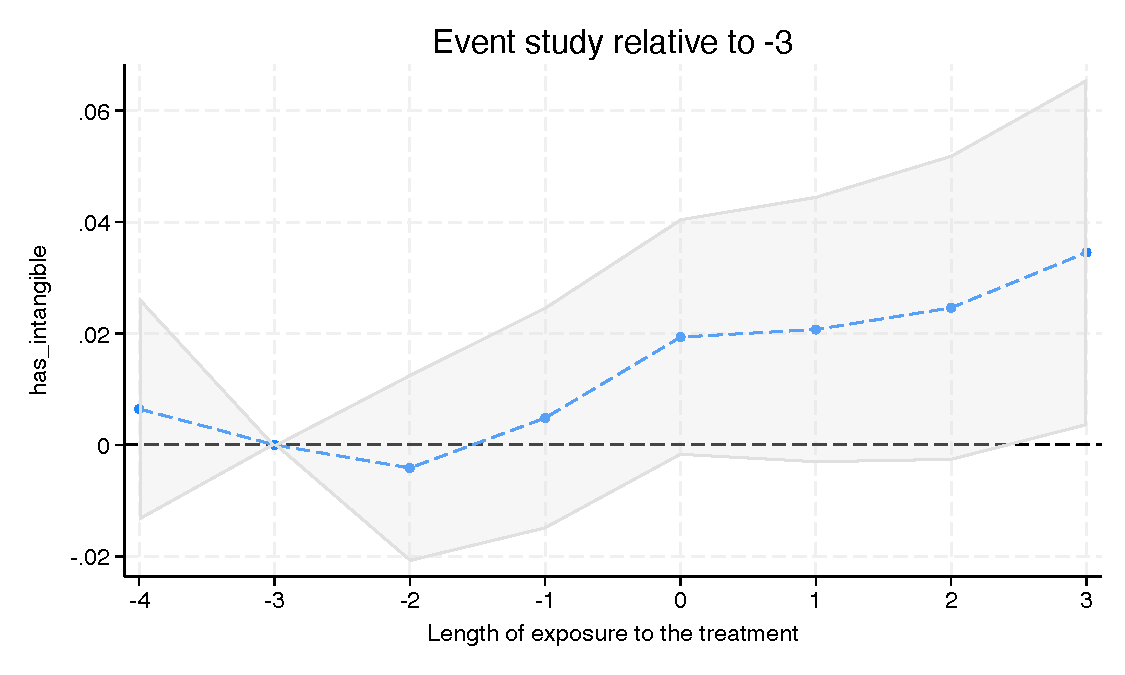
\includegraphics[width=0.8\textwidth]{figure/event_study_has_intangible.pdf}
\caption{Evolution of Intangible Assets Under Good vs Bad CEOs}
\label{fig:intangibles}
\end{figure}

The contrasting dynamics between materials and capital provide compelling evidence for our framework. Figure \ref{fig:materials} shows that material purchases jump immediately by [[immediate materials jump]] percent in year 0 under good CEOs, consistent with managers having direct control over input purchases. Meanwhile, capital shows no discontinuous change at the transition point, confirming physical investment remains under owner control.

\begin{figure}[htbp]
\centering
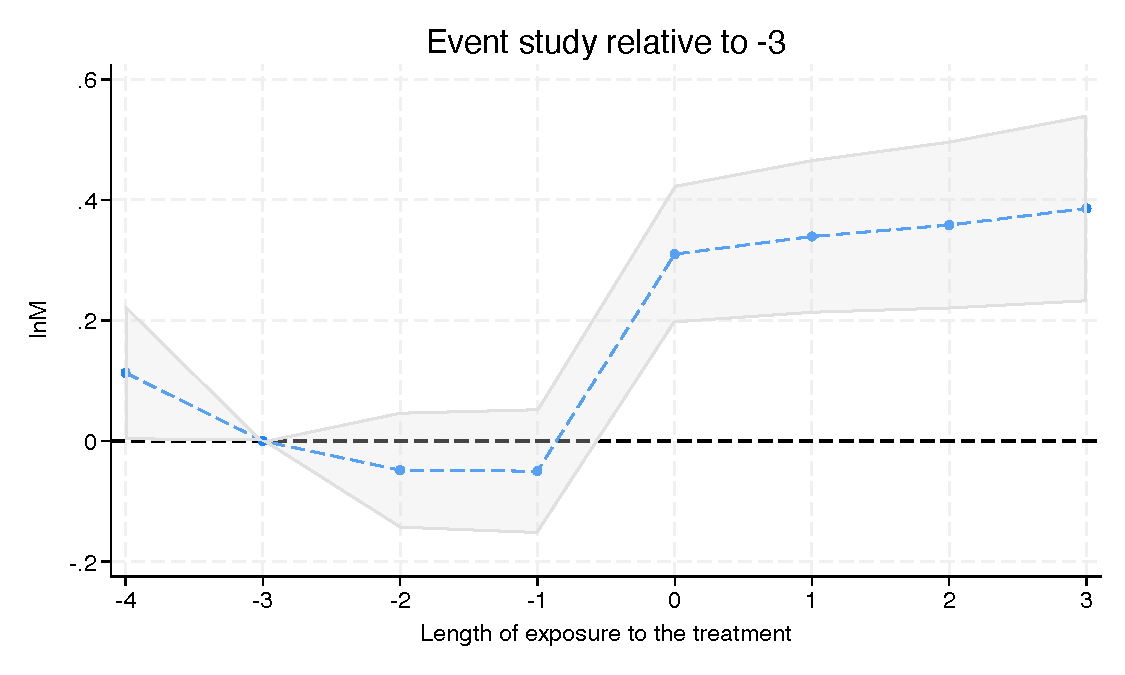
\includegraphics[width=0.8\textwidth]{figure/event_study_lnM.pdf}
\caption{Immediate Adjustment of Material Inputs Under New CEOs}
\label{fig:materials}
\end{figure}

These differential effects across outcomes—immediate for manager-controlled variables, gradual or absent for owner-controlled ones—support our model's division of decision rights and strengthen the causal interpretation of our estimates.

This division of control aligns with evidence from multi-plant firms where plant managers in family-owned businesses face constraints on capital investment, innovation, and marketing decisions but maintain autonomy over labor hiring \citep{bloom2012americans}. The pattern also reflects broader governance structures in concentrated ownership firms where owners preserve strategic control while delegating operational management \citep{zellweger2012managing}.

\section{Conclusion}

Our main finding: three-quarters of apparent CEO effect is spurious. The naive comparison of firms hiring good versus bad CEOs suggests a [[raw CEO gap]] percent performance difference. Our placebo-controlled event study reveals [[placebo gap]] percent of this gap arises from mechanical noise in fixed effects estimation. The true causal effect is [[true CEO effect]] percent—a quarter of what raw correlations suggest.

CEOs matter modestly, with their primary impact through scaling variable inputs. Better managers expand operations by immediately increasing employment and material purchases, generating higher revenues within the constraints of owner-controlled capital. The [[true CEO effect]] percent productivity advantage translates into [[revenue effect]] percent higher revenues through this scaling mechanism. The immediate response of manager-controlled variables contrasted with unchanged capital stocks validates our model's division of decision rights.

These findings have implications for corporate governance and productivity research. The widespread practice of using manager fixed effects as explanatory variables is flawed—with [[percent noise]] percent noise contamination, such estimates suffer from severe attenuation bias. This explains the weak and inconsistent relationships found in studies relating manager "quality" to firm policies or outcomes. Researchers should not trust raw CEO fixed effects as measures of managerial ability.

Future research should use observable manager characteristics. Education and work experience \citep{DePirro2025}, foreign name as a proxy for international exposure \citep{Koren2023expat}, and selectiveness of entry cohorts \citep{koren2024managers} offer more reliable, though narrower, measures of specific dimensions of managerial quality. These observables capture only partial aspects of CEO ability but avoid the mechanical noise that contaminates fixed effects estimates.

Our placebo-controlled approach offers a general solution for short-panel settings where traditional methods fail. This extends beyond CEOs to teachers, doctors, judges, or any setting where individual effects are estimated from limited observations. The method requires only the ability to construct credible placebo treatments—randomly splitting stable spells in our case—making it widely applicable. Rather than attempting complex analytical corrections that become unreliable with few observations, the placebo approach directly measures and removes the noise component.

Our findings offer both methodological and substantive contributions. The placebo control technique provides a practical tool for future research on manager effects, applicable beyond our specific context. For policy, the modest but real CEO effects suggest that while management quality matters, other factors—organizational capital, market position, ownership structure—play larger roles in firm performance. Understanding this balance helps calibrate expectations about what management improvements can realistically achieve in private businesses.

[[Note: Add final big-picture paragraph discussing broader implications for understanding productivity differences across firms, the role of management in economic development, and how our findings reconcile conflicting evidence in the literature about the importance of management.]]

\bibliographystyle{apalike}
\bibliography{references}

\appendix

\section{Additional Tables and Figures}

[[insert surplus share table here]]

[[insert additional revenue function specifications here]]

\subsection{Variance-Based Evidence for CEO Heterogeneity}

[[Note: Move variance event study here as Figure A1]]

Figure \ref{fig:variance_event_study} presents complementary evidence using the variance of log TFP around CEO transitions. Under our framework, if CEO changes introduce real heterogeneity in managerial quality, the cross-sectional variance of outcomes should increase at the transition point—some firms get better CEOs, others get worse ones. In contrast, pure noise or firm-specific trends would not systematically alter variance.

[[Note: Insert figure showing variance jumps for actual transitions but remains flat for placebo transitions]]

[[Note: Describe how variance increases by X% at actual CEO transitions and remains elevated, while placebo transitions show no change in variance, providing model-free evidence that CEO transitions introduce real heterogeneity]]

\section{Robustness Checks}

We conduct extensive robustness checks to validate our main findings. Table [[robustness table]] presents placebo-controlled estimates across different specifications and samples.

\subsection{Alternative Outcome Variables}

Beyond revenue, we examine log wage bill and log materials as outcomes. The placebo-controlled effects remain consistent: good CEOs increase the wage bill by [[wage bill effect]] percent and materials by [[materials effect]] percent, with [[placebo wage bill]] and [[placebo materials]] percent arising from noise respectively.

\subsection{Sectoral Heterogeneity}

Revenue function parameters vary across sectors, with manufacturing showing higher capital elasticities than services. Despite these differences, the placebo-controlled CEO effect remains remarkably stable at [[sectoral range]] percent across industries, suggesting our findings are not driven by sector-specific dynamics.

\subsection{Sample Restrictions}

We test sensitivity to sample definitions:

\begin{enumerate}
\item \textbf{Post-2004 only}: Restricting to the post-EU accession period yields a [[post 2004 effect]] percent effect, confirming results are not driven by the transition economy period.

\item \textbf{Lower size threshold}: Including firms with 2+ employees (rather than 5+) increases the raw effect to [[lower threshold raw]] percent but also increases noise to [[lower threshold placebo]] percent, yielding a similar true effect of [[lower threshold true]] percent.

\item \textbf{Excluding founders}: When we exclude founder-managed firms from the event study, the true effect increases to [[no founder effect]] percent, suggesting founders may have non-pecuniary objectives that reduce measured productivity.

\item \textbf{Connected component only}: Restricting to the largest connected component yields [[connected only effect]] percent, nearly identical to the full sample.

\item \textbf{Including small components}: Including all connected components (even those with fewer than 10 managers) produces [[all components effect]] percent, confirming our results are not sensitive to component size restrictions.
\end{enumerate}

These robustness checks confirm that our central finding—three-quarters of apparent CEO effects are noise—holds across different samples, outcomes, and specifications.

\end{document}


\subsection{Empirical Specification}

To estimate manager effects from observational data, we substitute unobserved prices and organizational capital with fixed effects:
\begin{equation}\label{eq:empirical}
r_{imst} = \frac{\alpha}{\chi} k_{it} + \frac{1}{\chi}z_m + \lambda_i + \mu_{st} + \tilde{\epsilon}_{it}
\end{equation}
where $\lambda_i = a_i/\chi$ captures time-invariant firm characteristics, $\mu_{st}$ absorbs sector-time variation in prices, and $\tilde{\epsilon}_{it} = \epsilon_{it}/\chi$ is rescaled residual productivity.

The key identifying assumption is that residual productivity $\tilde{\epsilon}_{it}$ is uncorrelated with manager assignment conditional on firm and sector-time fixed effects. This allows manager skills and physical capital to be arbitrarily correlated with firm quality and market conditions—better firms may hire better managers and invest more. We only require that the residual variation in productivity is orthogonal to manager assignment.

\subsection{Challenges in Estimating Manager Effects}

Three challenges complicate estimating manager effects from equation \eqref{eq:empirical}:

First, residual productivity $\tilde{\epsilon}_{it}$ may correlate with manager changes if firms replace CEOs in response to productivity shocks. This reverse causality biases estimates of manager effects.

Second, manager fixed effects are only identified for the connected set of firms and managers linked through mobility. Effects are measured relative to a reference group within each connected component, limiting comparability across components.

Third, estimated manager effects $\hat{z}_m$ include both true skill and averaged residual productivity: $\hat{z}_m = z_m + \bar{\epsilon}_{im}$ where $\bar{\epsilon}_{im}$ is the average $\tilde{\epsilon}_{it}$ during manager $m$'s tenure at firm $i$. When managers have short tenures, this noise component dominates the signal, making raw fixed effects unreliable measures of true skill.

When CEO $m$ manages firm $i$ for $T_{im}$ years, the estimated effect is $\hat{z}_m = z_m + \frac{1}{T_{im}}\sum_t \epsilon_{it}$. With median tenure of [[median tenure]] years and i.i.d. shocks, the noise-to-signal ratio is proportional to $1/\sqrt{T_{im}}$, making noise dominate for typical tenures. This mechanical bias affects all fixed effects estimates but becomes particularly severe in CEO settings where individual observations are limited.

Our placebo-controlled approach addresses these challenges by measuring and removing the noise component from estimated manager effects.
